

\section{Trær}
Et tre en et spesielt tilfelle av en rettet graf der hver node har inngrad 1 (med unntak av rota i treet). Vi ser på et eksempel:
\begin{figure}[H]
\caption{Et lite binært tre}
\label{fig:tre}
\centering
~\\
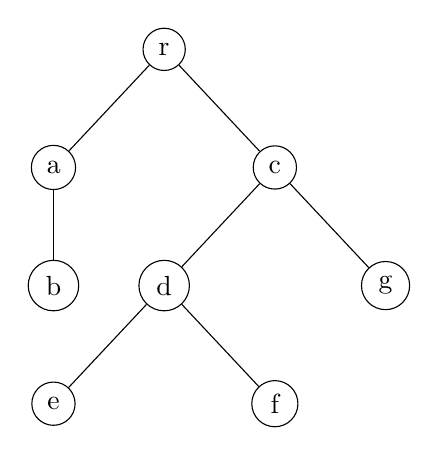
\begin{tikzpicture}[sibling distance=8em,
every node/.style = {shape=circle, draw, align=center}]

\node{r}
	child {node {a}
		child {node {b}}
	}
	child {node {c}
		child {node {d}
			child {node {e}}
			child {node {f}}
		}
		child {node {g}}
	};
\end{tikzpicture}
\end{figure}

\paragraph{Terminologi}~\\
Vi skal se litt på ord og uttrykk for trær. Gjennomgående bruker vi treet i figur \ref{fig:tre} som eksempel

I figuren blir nodene tegnet som rundinger. For å betegne relasjonen mellom nodene bruker vi ofte familierelasjoner. Vi sier at $ e $ og $ f $ er \textbf{søsken}, $ d $ er \textbf{forelder} til $ e $, og $ e $ er \textbf{barn} av $ d $. Vi kan også si at $ g $ er \textbf{onkel} til $ f $, men dette er mindre vanlig, da vi sjeldent har bruk for å snakke om \say{onkelnoder}. 

Nodene $ r, a, c $ og $ d $ kalles \textbf{indre noder}, det vil si at disse nodene har barn. Noder som ikke har noen barn kalles \textbf{løvnoder}

I figur \ref{fig:tre} er $ r $ \textbf{rotnoden}. Rota i treet er den eneste noden uten noen foreldre. Rota er derfor et naturlig startpunkt når vi skal søke eller traversere gjennom treet. 


\subsection{Binære søketrær}
\label{bintraer}
Binære søketrær er trær med noen spesielle krav. Hver node kan ikke ha mer enn to barn, vi kaller dem ofte venstre og høyre barn. Venstre barn er alltid mindre enn noden selv, og høyre barn er alltid større enn noden. Dette gjør binære søketrær meget godt egnet for søking. 

\begin{teorem}
\label{teo:bintre}
Å sette inn, fjerne eller søke etter noder i et binært søketre har
\begin{enumerate}[i]
\item I beste fall $ O(\log n) $ tid
\item I verste fall $ O(n) $ tid
\end{enumerate}
\end{teorem}

Vi skal ikke bevise teorem \ref{teo:bintre} her\footnote{Det kan vises ved induksjon at høyden til et binært tre i beste fall er $ \log_2 n $}, men vi kan se på et eksempel som viser ytterpunktene. I figur \ref{fig:bintre} ser vi to forskjellige binære søketrær. I treet til venstre har vi et fint, balansert tre. Det er lett å se at høyden (og dermed antall operasjoner vi må gjøre for å komme til bunn i treet) er lik $ \lceil \log_2 n \rceil $ der $ n $ er antall noder i treet.

I treet til høyre har hver node kun ett barn. Vi har i praksis en lenkeliste. Hvis vi skal søke etter 4, må vi tråkke gjennom alle de andre nodene for å komme dit. 

\begin{figure}[H]
\caption{To eksempler på binære søketrær}
\label{fig:bintre}
\centering
~\\
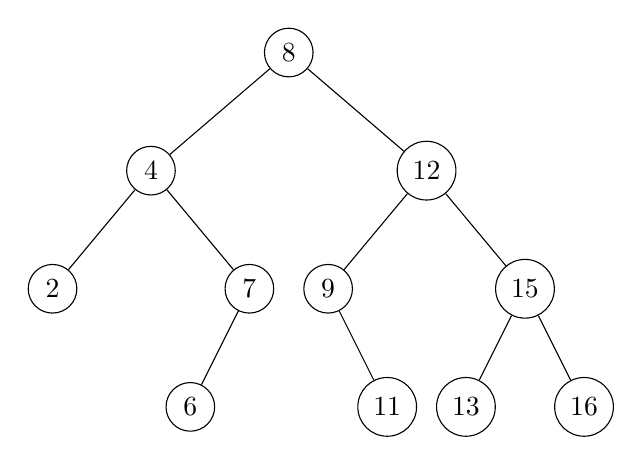
\begin{tikzpicture}[level distance=1.5cm,
  level 1/.style={sibling distance=3.5cm},
  level 2/.style={sibling distance=2.5cm},
  level 3/.style={sibling distance=1.5cm},
every node/.style = {shape=circle, draw, align=center}]

\node{8}
	child {node {4}
		child {node {2}}
		child {node {7}
			child {node {6}}
			child [missing]{}
		}
	}
	child {node {12}
		child {node {9}
			child [missing]{}
			child {node {11}}
		}
		child {node {15}
			child {node {13}}
			child {node {16}}
		}
	};
\end{tikzpicture}
$ \quad\quad $
\begin{tikzpicture}[level distance=1.5cm,sibling distance=2cm,
every node/.style = {shape=circle, draw, align=center}]

\node{1}
	child [missing] {}
	child {node {2}
		child [missing]{}
		child {node {3}
			child [missing]{}
			child {node {4}}
		}
	};
\end{tikzpicture}
\end{figure}




\paragraph{Innsetting}~\\
Når vi skal sette inn en node i et binært søketre starter vi i rota. Vi sammenligner verdien vi skal sette inn med verdien i rota. Hvis verdien vi setter inn er mindre enn rota går vil til venstre, er den større går vi til høyre. Hva som skjer ved likhet er opp til oss å bestemme, men vi må være konsekvente. Når vi kommer til en nullpeker kan vi sette denne pekeren til å peke på noden vi setter inn.

Vi kan implementere denne funksjonen rekursivt. I en ytre klasse kan vi skrive en skallfunksjon som kaller på rotas \verb|instert|-metode. Vi har en indre \verb|Node|-klasse med en rekursiv insertmetode. Den kan implementeres slik:
\javaimport{kode/ex_bintree_insert.java}


\paragraph{Fjerning}~\\
Når vi skal fjerne en node fra et binært søketre har vi tre forskjellige situasjoner som vi må se på.

{\bfseries Noden har ingen barn} (løvnode). Denne situasjonen er ganske grei. Siden noden ikke har noen barn å forholde seg til er det bare å fjerne den fra treet.

{\bfseries Noden har ett barn}. For å fjerne en node $ a $ med ett barn kan vi ganske enkelt flytte pekeren fra foreldernoden til $ a $, til barnet til $ a $.

{\bfseries Noden har to barn}. Hvis noden vi skal fjerne har to barn tar vi opp den minste noden som er større en noden vi skal fjerne og flytter den til den posisjonen noden vi skulle fjærne var. Vi finner den minste noden som er større ved å gå ett steg til høyre, og så til venstre helt til vi er i bunn av treet. 

Eksempel på implementasjon i Java (rekursiv metode i en \verb|Node|-klasse):
\javaimport{kode/ex_bintree_remove.java}


\paragraph{Søking}~\\
Når vi skal søke etter et element i et søketre starter vi i rota og sammenligner det elementet vi søker etter med det elementet som finnes i rota. Er elementet vår mindre enn noden vi ser på går vi til venstre, og er det større går vi til høyre. Deretter foretar vi samme testen på nytt og fortsetter slik til vi enten finner elementet vi leter etter, eller kommer til en nullpeker (bunnen av treet).

Eksempel på implementasjon i Java:
\javaimport{kode/ex_bintree_search.java}





~\\~\\
\subsection{Rød-svarte trær} \label{rb_tre}
Rødsvarte trær er binære søketrær med noen spesielle strukturkrav. Kravene er designet for å motkjempe skjevhet (som illustrert i figur \ref{fig:bintre}), og dermed forbedre kjøretid.

Vi deler nodene opp i to kategorier, røde og svarte. Vi følger noen bestemte regler på hvordan vi skal farge nodene, og fargen på nodene avgjør som vi må benytte oss av rotasjon eller ikke (se \ref{trerotasjon}). Fargen til en node er \textbf{ikke} statisk, den kan endres.

\begin{definisjon}
\label{def:rb_tree}
Et rød-svart tre er et binært søketre der hver node er
farget enten rød eller svart slik at:
\begin{enumerate}[i]
\item Roten er svart.
\item Hvis en node er rød, må barna være svarte.
\item Enhver vei fra en node til en null-peker må inneholde samme antall svarte noder.
\end{enumerate}
\end{definisjon}

Dette sikrer at høyden maksimalt er $ 2\log_2 (n+1) $

\paragraph{Insetting}~\\
For å sette inn en node i rød-svarte trær kan vi bruke algoritmen i teorem \ref{teo:ins_rb}
\begin{teorem} Innsetting i rød-svarte trær. \label{teo:ins_rb}

La $ N $ være noden vi ønsker å sette inn i treet. La $ P $ være forelder, $ G $ besteforelder, og $ U $ onkel til $ N $. Følgende algoritme vil da gi en korrekt innsetting i et rød-svart tre:
\begin{enumerate}
\item Gjør innsetting som i vanlig binært søketre, der $ N $ farges rød.
\item Hvis $ N $ er rota i treet: farg $ N $ svart. 
\item Hvis $ P $ er svart: alt OK. Innsetting ferdig. 
\item Hvis $ P $ er rød og $ N $ ikke er rot:
	\begin{enumerate}
		\item Hvis $ U $ er svart:
		\begin{enumerate}
			\item Farg $ P $ svart
			\item Farg $ G $ rød
			\item Repeter fra pt. 2 med $ G $ som $ N $
		\end{enumerate}
		\item Hvis $ U $ er rød:
		\begin{enumerate}
			\item $ N $ er venstre barn av $ P $, som er venstre barn av $ G $:\\
			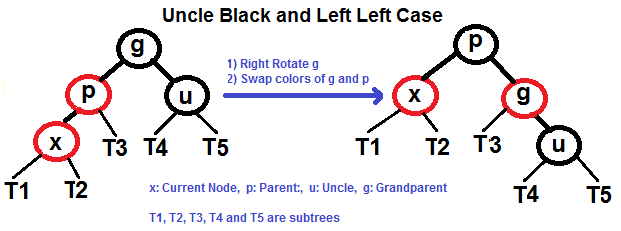
\includegraphics[width=0.65\textwidth]{fig/rbt_ll.png}\\

			\item $ N $ er høyre barn av $ P $, som er venstre barn av $ G $:\\
			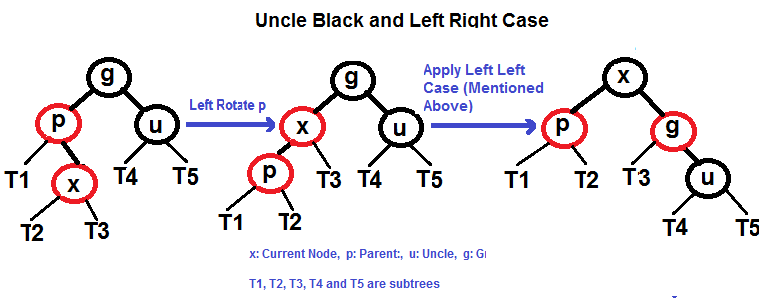
\includegraphics[width=0.65\textwidth]{fig/rbt_lr.png}\\
			
			\item $ N $ er høyre barn av $ P $, som er høyre barn av $ G $ (speilvendt av i):\\
			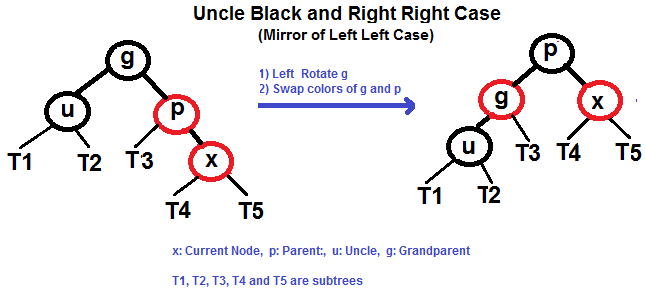
\includegraphics[width=0.65\textwidth]{fig/rbt_rr.png}\\
			
			\item $ N $ er venstre barn av $ P $, som er høyre barn av $ G $ (speilvendt av ii):\\
			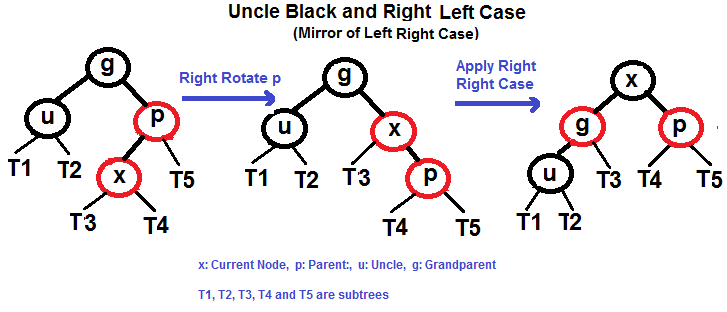
\includegraphics[width=0.65\textwidth]{fig/rbt_rl.png}\\
			
		\end{enumerate}
	\end{enumerate}
\end{enumerate}
\end{teorem}


\paragraph{Fjerning}~\\
Vi skal fjerne en node $ N $ fra et rød-svart tre.

Vi ser på noen spesialtifeller: Hvis $ N $ er en rød node er jobben enkel. Vi sletter da $ N $ som om vi hadde et vanlig søketre. Det samme gjelder hvis forelderen til $ N $ er rød og $ N $ er eneste barn. Hvis $ N $ er svart og har ett barn sletter vi $ N $ og farger barnet svart. 

Generelt sletter vi noden som i et vanlig binært søketre, og utfører nødvendige rotasjoner og omfarginger for å beholde kravet i definisjon \ref{def:rb_tree}.


\paragraph{Tidsanalyse}~\\
Siden høyden til et rød-svart tre maksimalt er $ 2\log_2 (n+1) $ har vi worst case tid $ O(\log_2 n) $. Selv om vi risikerer å måtte gjøre rotasjoner er innsetningstiden også $ O(\log_2 n) $.


~\\
\subsection{B-trær} \label{b-tre}
B-trær er konstruert for å effektivisere antall disklesninger, og gir mening å bruke hvis vi har et tre som er så stort at det må lagres på gammeldagse spinnedisker, og ikke i RAM. Vi lagrer dataene i blokker, og leser en og en blokk av gangen. Alle dataene er lagret i løvnodene, mens de indre nodene brukes for søking. En vanlig måte å implementere B-trær på er å ha så mye av toppen i RAM som mulig, og lagre resten på disk. B-trær er ikke binære, dvs at de kan ha flere enn 2 barn. 

\begin{definisjon} La $ M $ angi antall mulige nøkler i hver indre node, og $ L $ angi maksimalt antall dataelementer i hver løvnode. B-trær er søketrær der følgende kriterier er oppfylt:
\begin{enumerate}[i]
\item Alle dataene er lagret i løvnodene
\item Interne noder lagrer inntil $ M-1 $ nøkler for søking: nøkkel $ i $ angir den minste verdien i subtre $ i+1 $.
\item Roten er enten en løvnode, eller har mellom 2 og $ M $ barn. 
\item Alle andre indre noder har mellom $ \lceil M/2\rceil $ og $ M $ barn. 
\item Alle løvnoder har samme dybde.
\item Alle løvnoder har mellom $ \lceil L/2\rceil $ og $ L $ dataelementer
\end{enumerate}
\label{def:b_tre}
\end{definisjon}


\paragraph{Innsetting}~\\
Når vi skal sette inn et element i et B-tre finner vi plassen elementet skal på, og setter det der. Hvis løvnoden vi setter elementet inn i er full må vi splitte noden i to like store deler. Vi må da oppdatere nøklene i foreldrenoden $ P $. Hvis $ P $ ikke har plass til en ekstra nøkkel må vi splitte den også, og oppdatere nøklene i foreldrenoden til $ P $. Slik fortsetter vi oppover til vi får en node som har plass til en ekstra nøkkel. Den eneste måten et B-tre kan øke høyden på er at rota splittes i to, og at vi lager en ny rot. 

\begin{eks} Sett inn 13 og 42 i følgende B-tre ($ M = 3 $ og $ N = 4 $):
\begin{figure}[H]
\centering
\begin{tikzpicture}
[level distance=1.5cm,
  level 1/.style={sibling distance=4cm},
  level 2/.style={sibling distance=1.3cm},
every node/.style = {align=center}]
\tikzstyle{inner} = [ellipse, draw=black]
\tikzstyle{leaf} = [rectangle, draw=black]

\node[inner] {17; -}
child {
	node[inner] {12; - }
	child {
		node[leaf] {2\\3\\6\\~}
	}
	child {
		node[leaf] {12\\14\\~\\~}
	}
	child[missing]
}
child {
	node[inner] {33; -}
	child {
		node[leaf] {17\\18\\29\\30}
	}
	child {
		node[leaf] {33\\37\\40\\41}
	}
	child[missing]
}
;

\end{tikzpicture}
\end{figure}

Vi starter med å sette inn 13. Vi ser først på rota: (17; -). 13 er mindre enn 17, så vi går til første barn. Så sammenligner vi med (12; -). 13 er sørre enn 13, og mindre enn uendelig (- symboliserer minste verdi i tredje barn, men siden det barnet ikke eksisterer tenker vi på verdier som $ \infty $). Vi går derfor til andre barn. Der ser vi at vi kan sette inn 13 uten problemer. 

Vi skal nå sette inn 42. 42 er større enn 33 så vi går til andre barn. Igjen er 42 større enn 33 så vi går til andre barn igjen. Her ser vi at hvis vi legger til 42 i bunn av noden (33, 37, 40, 41) blir størrelsen lik 5, altså større enn $ N $. Vi må splitte noden. Når vi splitter en node med et odde antall elementer er det ikke helt klart som vi skal ta med oss størsteparten, eller la størsteparten være igjen. I dette tilfellet vil vi få en node med 3 og en node med 2 elementer. Vi kan selv velge om den nye noden skal ha 2 eller 3 elementer, men vi må være konsekvente. I dette tilfellet lar vi den nye noden ha 2 elementer. Vi oppdaterer foreldrenoden. Siden den har to barn fra før og $ M=3 $ går det fint, vi trenger ikke splitte videre oppover. 

Resultatet etter innsetting ser slik ut:

\begin{figure}[H]
\centering
\begin{tikzpicture}
[level distance=1.5cm,
  level 1/.style={sibling distance=4cm},
  level 2/.style={sibling distance=1.3cm},
every node/.style = {align=center}]
\tikzstyle{inner} = [ellipse, draw=black]
\tikzstyle{leaf} = [rectangle, draw=black]

\node[inner] {17; -}
child {
	node[inner] {12; - }
	child {
		node[leaf] {2\\3\\6\\~}
	}
	child {
		node[leaf] {12\\13\\14\\~}
	}
	child[missing]
}
child {
	node[inner] {33; 41}
	child {
		node[leaf] {17\\18\\29\\30}
	}
	child {
		node[leaf] {33\\37\\40\\~}
	}
	child {
		node[leaf] {41\\42\\~\\~}
	}
}
;

\end{tikzpicture}
\end{figure}
\end{eks}

~\\
\paragraph{Fjerning}~\\
Hvis vi skal fjerne et element fra et B-tre søker vi opp elementet, tar det vekk, og hvis mengden elementer i noden blir mindre enn grensen satt i def. \ref{def:b_tre}.vi slår vi sammen to noder. Den eneste måten B-trær kan minke i høyde på er om alle barna til rota blir slått sammen til én node (vi fjerner da rota). 

\begin{eks} Fjern 41 fra følgende B-tre:

\begin{figure}[H]
\centering
\begin{tikzpicture}
[level distance=1.5cm,
  level 1/.style={sibling distance=4cm},
  level 2/.style={sibling distance=1.3cm},
every node/.style = {align=center}]
\tikzstyle{inner} = [ellipse, draw=black]
\tikzstyle{leaf} = [rectangle, draw=black]

\node[inner] {17; -}
child {
	node[inner] {12; - }
	child {
		node[leaf] {2\\3\\6\\~}
	}
	child {
		node[leaf] {12\\13\\14\\~}
	}
	child[missing]
}
child {
	node[inner] {33; 41}
	child {
		node[leaf] {17\\18\\29\\30}
	}
	child {
		node[leaf] {33\\37\\40\\~}
	}
	child {
		node[leaf] {41\\42\\~\\~}
	}
}
;

\end{tikzpicture}
\end{figure}
Vi ser at 41 er mellom 17 og $ \infty $, så vi går til andre barn. Deretter ser vi at 41 er større enn 33 og større enn eller lik 41. Vi går derfor til tredje barn og fjerner 41. Vi ser at da vi noden kun ha ett element, og vi slår den sammen med noden før. Resultatet etter fjerning blir
\begin{figure}[H]
\centering
\begin{tikzpicture}
[level distance=1.5cm,
  level 1/.style={sibling distance=4cm},
  level 2/.style={sibling distance=1.3cm},
every node/.style = {align=center}]
\tikzstyle{inner} = [ellipse, draw=black]
\tikzstyle{leaf} = [rectangle, draw=black]

\node[inner] {17; -}
child {
	node[inner] {12; - }
	child {
		node[leaf] {2\\3\\6\\~}
	}
	child {
		node[leaf] {12\\13\\14\\~}
	}
	child[missing]
}
child {
	node[inner] {33; -}
	child {
		node[leaf] {17\\18\\29\\30}
	}
	child {
		node[leaf] {33\\37\\40\\42}
	}
	child[missing]
}
;

\end{tikzpicture}
\end{figure}
\end{eks}



\paragraph{Tidsanalyse}

\begin{teorem} Å søke etter, sette inn og fjerne elementer fra et B-tre tar, både i beste og verste fall, $ O(\log n) $ tid.
\end{teorem}




\newpage
\subsection{Rotasjon}
\label{trerotasjon}

\subsubsection{Zig}
For å skjønne zig-rotasjon ser vi på en figur:

\begin{figure}[H]
\caption{Zig-rotasjon mhp X}
\centering
\begin{tikzpicture}[level distance=1.5cm,
  level 1/.style={sibling distance=2cm},
  level 2/.style={sibling distance=1.3cm}]

\tikzstyle{subtree} = [isosceles triangle, draw=black, align=center, minimum height=0.5cm, minimum width=1cm, shape border rotate=90, anchor=center]
\tikzstyle{n} = [draw=black, draw=black, align=center, circle]

\node[n] {P}
child {
	node[n] {X}
	child {
		node[subtree] {A}
	}
	child {
		node[subtree] {B}
	}
}
child {
	node[subtree] {C}
}
;
\end{tikzpicture}
\quad\raisebox{5\height}{\scalebox{2}{$\rightarrow$}}\quad
\begin{tikzpicture}[level distance=1.5cm,
  level 1/.style={sibling distance=2cm},
  level 2/.style={sibling distance=1.3cm}]

\tikzstyle{subtree} = [isosceles triangle, draw=black, align=center, minimum height=0.5cm, minimum width=1cm, shape border rotate=90, anchor=center]
\tikzstyle{n} = [draw=black, draw=black, align=center, circle]

\node[n] {X}
child {
	node[subtree] {A}
}
child {
	node[n] {P}
	child {
		node[subtree] {B}
	}
	child {
		node[subtree] {C}
	}
}
;
\end{tikzpicture}
\end{figure}

En zig-rotasjon vil beholde egenskapene til et binært søketre siden alle nodene i A er mindre enn X og P, alle nodene i B er større enn X og mindre enn P, og alle nodene i C er større enn både X og P. Vi ser at alle høyre barn av P også er høyre barn av P \emph{etter} rotasjonen, etc. 

Vi har også noe som heter zig-zig-rotasjon, som er å utføre en zig-rotasjon to ganger.


\subsubsection{Zig-zag}
Igjen ser vi på en figur:

\begin{figure}[H]

% Dette er helt forferdelig kode. Jeg vet, og jeg beklager. 

\caption{Zig-zag-rotasjon mhp X:}
\centering
\begin{tikzpicture}[level distance=1.5cm,
  level 1/.style={sibling distance=2cm},
  level 2/.style={sibling distance=1.3cm}]

\tikzstyle{subtree} = [isosceles triangle, draw=black, align=center, minimum height=0.5cm, minimum width=1cm, shape border rotate=90, anchor=center]
\tikzstyle{n} = [draw=black, draw=black, align=center, circle]

\node[n] {G}
child {
	node[n] {P}
	child {
		node[subtree] {A}
	}
	child {
		node[n] {X}
		child {
			node[subtree] {B}
		}
		child {
			node[subtree] {C}
		}
	}
}
child {
	node[subtree] {D}
}
;
\end{tikzpicture}
\quad\raisebox{9\height}{\scalebox{2}{$\rightarrow$}}\quad
\raisebox{.25\height}{
\begin{tikzpicture}[level distance=1.5cm,
  level 1/.style={sibling distance=2.7cm},
  level 2/.style={sibling distance=1.3cm}]

\tikzstyle{subtree} = [isosceles triangle, draw=black, align=center, minimum height=0.5cm, minimum width=1cm, shape border rotate=90, anchor=center]
\tikzstyle{n} = [draw=black, draw=black, align=center, circle]

\node[n] {X}
child {
	node[n] {P}
	child {
		node[subtree] {A}
	}
	child {
		node[subtree] {B}
	}
}
child {
	node[n] {G}
	child {
		node[subtree] {C}
	}
	child {
		node[subtree] {D}
	}
}
;
\end{tikzpicture}
}
\end{figure}

Som i tilfellet med zig-rotasjon ser vi at egenskapene til et binært søketre er bevart. 